\begin{frame}
  \frametitle{Ustálený stav}
  
    \begin{multline*}
    \frac{1}{v(E)} {\pd{\angflux(\br,E,\bomega,t)}{t}} = \\
    {P(\br,E,\bomega,t)}
    - {\Sigma_t(\br,E,\bomega,t)\angflux(\br,E,\bomega,t)}
    - {\bomega\cdot\nabla\angflux(\br,E,\bomega,t)}
    \end{multline*}
    + počáteční a okrajové podmínky
    \uncover<2>{
    \begin{center}
    \begin{tikzpicture}
      \draw[decorate, decoration=snake,thick,structure,->] (0,0) -- (0,-1);
    \end{tikzpicture}
    \end{center}
    $$
      \bomega\cdot\nabla\angflux(\br,E,\bomega) +
      \Sigma_t(\br,E,\bomega)\angflux(\br,E,\bomega) =
      P(\br,E,\bomega)
    $$
    \\[.5em]
    + okrajové podmínky
    }

\end{frame}

\begin{frame}
  \frametitle{Operátorový zápis}
  \framesubtitle{integro-diferenciální LBR}
  
$$
  \left\{
    \begin{aligned}
       \alert<2-3>{L\angflux} &= P \equiv \alert<4>{H\angflux} + \alert<5>{F\angflux} + \alert<6>{Q}\quad &&\mbox{ v $X$,}\\
	  \angflux  &= \alert<7>{\beta\angflux} + \angfluxin\quad   &&\mbox{ na $\pX[-]$.}
    \end{aligned}
  \right.
$$
\begin{itemize}
	\item<2-> \alert<2>{advekce} a \alert<3>{záchyt}: $(\alert<2-3>{L\angflux})(x) = \alert<2>{\bomega\cdot\nabla\angflux(x)} + \alert<3>{\Sigma_t\angflux(x)}$
	\item<4-> \alert<4>{rozptyl} a \alert<5>{stěpení}: 
	    \begin{align*}
		      (\alert<4>{H\angflux})(x) &= \aintp{\eintp{\Sigma_s(\br, E'\ra E, \bomega'\cdot\bomega)\angflux(\br,E',\bomega')}}\\
		      (\alert<5>{F\angflux})(x) &= \frac{1}{4\pi}\eintp{\nu\Sigma_f(\br, E'\ra E)\aintp{\angflux(\br,E',\bomega')}}
      \end{align*}
	\item<6-> \alert<6>{stálý vnější neutronový zdroj:} $\alert<6>{Q(x)}$
	\item<7-> \alert<7>{přestup přes okraje:}
	$$
		(\alert<7>{\beta\angflux})(x) = \bndint[']{\pX[+]}\beta(\br'\ra \br, E'\ra E, \bomega'\ra\bomega)\angflux(\br', E', \bomega')
  $$
\end{itemize}

\end{frame}

\begin{frame}
  \frametitle{Úloha na $\keff$}
  
  $$
  \left\{
    \begin{aligned}
       (L-H)\angflux &= \frac{1}{\keff} F\angflux &&\mbox{ v $X$,}\\
	  \angflux  &= \beta\angflux \quad   &&\mbox{ na $\pX[-]$.}
    \end{aligned}
  \right.
$$

\end{frame}

\begin{frame}
  \frametitle{Mnohagrupová integro-diferenciální LBR}
  
  \vspace{-1.25em}
  
  \hbox{}\hfill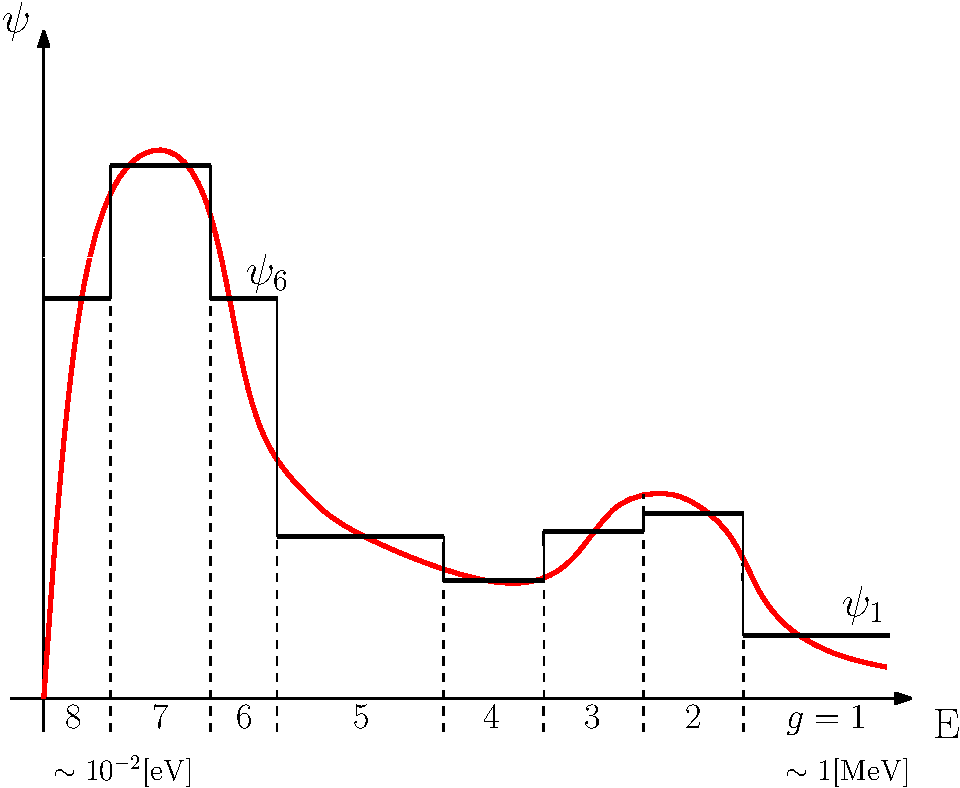
\includegraphics[width=.425\textwidth]{obr/fluxg}\hfill
  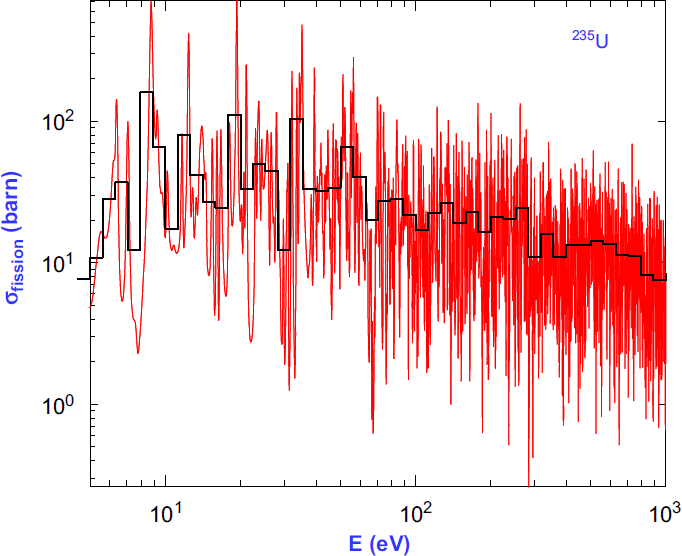
\includegraphics[width=.425\textwidth]{obr/U235fg}\hfill\hbox{}
  
  \shorten{-.6em}{0em}

  $$
  \left\{
    \begin{aligned}
    \llop\vangflux &= \hhop\vangflux + \ffop\vangflux + \QQ\quad &&\mbox{ v $X$,}\\
    \vangflux  &= \valbedo\vangflux + \vangflux_{\mathrm{in}}\quad   &&\mbox{ na $\pX[-]$}.
  \end{aligned}
  \right.
  $$

  \begin{gather*}
    \vangflux = \big[\angflux_g\big]_{g=1,\ldots, G}\quad
    \vangflux_{\mathrm{in}} = \big[\angflux_{\mathrm{in},g}\big]_{g=1,\ldots, G}\quad
    \QQ = \big[Q_g\big]_{g=1,\ldots, G}\\[.3em] 
    \llop = \big\llbracket L_{gg} \big\rrbracket_{g=1,\ldots, G} \\[.2em]
    \hhop = \big\llbracket H_{gg'}\big\rrbracket_{g,g'=1,\ldots, G} \quad
    \ffop = \big\llbracket F_{gg'}\big\rrbracket_{g,g'=1,\ldots, G} \quad
    \valbedo = \big\llbracket \beta_{gg'}\big\rrbracket_{g,g'=1,\ldots, G}
  \end{gather*}
  
  \lengthen
    
\end{frame}

\begin{frame}
  \frametitle{Monoenergetická podoba}
  
\begin{itemize}
	\item $ G = 1$,~ $\angflux = \angflux(\br,\bomega)$
	\item advekce a záchyt: $(L\angflux)(\br,\bomega) = \bomega\cdot\nabla\angflux(\br,\bomega) + \Sigma_t(\br)\angflux(\br,\bomega)$
	\item rozptyl a stěpení: 
	    \begin{align*}
		      (H\angflux)(\br,\bomega) &= \aintp{\Sigma_s(\br, \bomega'\cdot\bomega)\angflux(\br,\bomega')}\\
		      (F\angflux)(\br,\bomega) &= \frac{1}{4\pi}\nu\Sigma_f(\br)\aintp{\angflux(\br,\bomega')} = \frac{1}{4\pi}\nu\Sigma_f(\br)\fl(\br)
      \end{align*}
	\item stálý vnější neutronový zdroj: $Q(\br,\bomega)$
	\item přestup přes okraje: 
	$$
		(\beta\angflux)(x) = \bndint[']{\pX[+]}\beta(\br'\ra \br,\bomega'\ra\bomega)\angflux(\br',\bomega').
  $$
\end{itemize}

\end{frame}

\begin{frame}
  \frametitle{Integrální tvar}
  
\begin{itemize}
  \item Nechť $s\in I$ parametrizuje dráhu letu paralelního svazku neutronů
  \item V kartézské soustavě: $\der{x}{s} = \bomega_x,\ \der{y}{s} = \bomega_y,\ \der{z}{s} = \bomega_z$
	\item<2-> Označme $\Gamma = \{\br\in\RR[3]: \br = \br(s),\ s\in I\}$ ~(\emph{\color{structure}charakteristika})
	\item<3-> Platí
	  \begin{columns}
	  \column{.75\textwidth}
	    \begin{align*}
	      \bomega\cdot\nabla\angflux &= \bomega_x\pd{\angflux}{x} + 
	      \bomega_y\pd{\angflux}{y} + \bomega_z\pd{\angflux}{z}\\
	      & = 
	      \der{x}{s}\pd{\angflux}{x} + \der{y}{s}\pd{\angflux}{y} + \der{z}{s}\pd{\angflux}{z}
	      = 
	      \der{\angflux}{s}
	    \end{align*}
	  \column{.25\textwidth}
	  \hspace{-1.25em}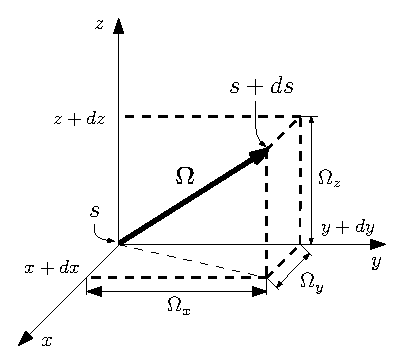
\includegraphics[width=1.15\textwidth]{obr/cartesian_streaming2}
	  \end{columns}\vspace{1em}
  \item<4-> $L\angflux \equiv \bomega\cdot\nabla\angflux + \Sigma_t\angflux = P\quad \Longrightarrow\quad \angflux = \alert<5>{L^{-1}}P$ \uncover<5->{\\(\alert<5>{umíme na charakteristikách})}
\end{itemize}

\end{frame}

\begin{frame}
  \frametitle{Integrální tvar}
  
  \begin{myitemize}
    \item Rovnice na charakteristice:~ $\der{\angflux(\br,\bomega)}{s} + \Sigma_t(\br,\bomega)\angflux(\br,\bomega) = P(\br,\bomega)$
    \item Řešení:~~ $\angflux(\br,\bomega) = \angflux(\br_0,\bomega)e^{-\tau(\br,\br_0)} + \int_0^{s_0} P(\br',\bomega)e^{-\tau(\br,\br')}\,\d{s'}$
    \begin{itemize}
    	\item $\br' = \br - s' \bomega$,~ $\br_0 = \br - s_0 \bomega$\\[.2em]
    	\item $\tau(\br,\br') = \tau(\br,\br-s'\bomega) = \int_0^{s'} \Sigma_t(\br - s''\bomega)\,\d{s''}$
    \end{itemize}
  \end{myitemize}
  \vspace{-.5em}
  \begin{center}
    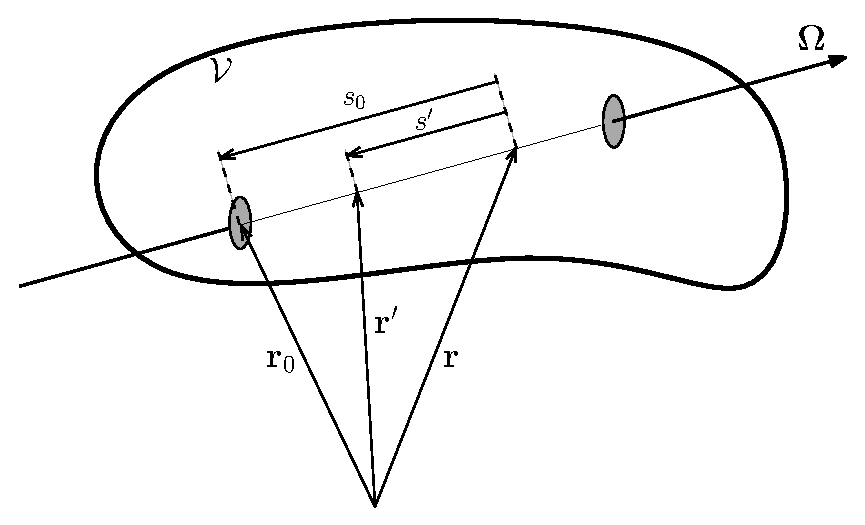
\includegraphics[scale=.5]{obr/trepka}
  \end{center}
  \vspace{-1em}
\end{frame}

\begin{frame}
  \frametitle{Integrální tvar}
  $$
    \angflux(\br,\bomega) = {\color<1>{red}\angflux(\br_0,\bomega)e^{-\tau(\br,\br_0)}} + {\color<2>{red}\int_0^{s_0} P(\br',\bomega)e^{-\tau(\br,\br')}\,\d{s'}}
  $$\\[1em]
  \ldots\ \alert<1>{neutrony, jež vstoupily do $\VV$ v $\br_0$ a dolétly do $\br$ (nebyly zachyceny)}\\
  $\hphantom{\ldots\ }$ + \alert<2>{neutrony ze zdrojů mezi $\br_0$ a $\br$, které nebyly zachyceny a dolétly do $\br$}\\
  $\hphantom{\ldots\ }$ (všechny uvažované neutrony letěly ve směru $\bomega$)
  \vspace{1em}
  \begin{itemize}[<3>]
    \item Na této formulaci jsou založeny např.
    \begin{itemize}
    	\item metoda charakteristik (MOC)
    	\item metoda kolizních pravděpodobností (CP)
    	\item nepřímo i metoda Monte Carlo (MC)
    \end{itemize}
  \end{itemize}


\end{frame}

\begin{frame}
  \frametitle{Trasování pohybu neutronů v integrálních metodách}
  \framesubtitle{Monte Carlo}
  \begin{center}
    \includegraphics<1>[scale=.5]{obr/MC}
    \includegraphics<2>[scale=.5]{obr/MC2}
  \end{center}
\end{frame}

\begin{frame}
  \frametitle{Trasování pohybu neutronů v integrálních metodách}
  \framesubtitle{Metoda (dlouhých) charakteristik}
  \vspace{-.4em}
  \begin{center}
    \includegraphics<1>[scale=.5]{obr/MOC}
    \includegraphics<2->[scale=.25]{obr/MOC2}
  \end{center}
  \only<2->{\vspace{-1.4em}}
  \begin{itemize}
    \only<1>{\item Geometrické informace (délky segmentů) lze spočíst nezávisle na $\angflux$}
  	\only<2->{\item Výpočet $\angflux_i(\bomega) = \Vint[\VV_i]{\angflux(\br,\bomega)}$ pro každou zónu nasčítáním příspěvků z jednotlivých charakteristik ve směru $\bomega$ (kvadratura pro prostor. int.)}
  	\item<3> Výpočet $\flux_i = \Vint{\flux(\br)}$ pro každou zónu nasčítáním $\angflux_i(\bomega)$ z charakteristik v jednotlivých směrech (kvadratura pro int. přes směry)
  \end{itemize}
  
\end{frame}


